\documentclass[twoside]{book}

% Packages required by doxygen
\usepackage{fixltx2e}
\usepackage{calc}
\usepackage{doxygen}
\usepackage[export]{adjustbox} % also loads graphicx
\usepackage{graphicx}
\usepackage[utf8]{inputenc}
\usepackage{makeidx}
\usepackage{multicol}
\usepackage{multirow}
\PassOptionsToPackage{warn}{textcomp}
\usepackage{textcomp}
\usepackage[nointegrals]{wasysym}
\usepackage[table]{xcolor}

% Font selection
\usepackage[T1]{fontenc}
\usepackage[scaled=.90]{helvet}
\usepackage{courier}
\usepackage{amssymb}
\usepackage{sectsty}
\renewcommand{\familydefault}{\sfdefault}
\allsectionsfont{%
  \fontseries{bc}\selectfont%
  \color{darkgray}%
}
\renewcommand{\DoxyLabelFont}{%
  \fontseries{bc}\selectfont%
  \color{darkgray}%
}
\newcommand{\+}{\discretionary{\mbox{\scriptsize$\hookleftarrow$}}{}{}}

% Page & text layout
\usepackage{geometry}
\geometry{%
  a4paper,%
  top=2.5cm,%
  bottom=2.5cm,%
  left=2.5cm,%
  right=2.5cm%
}
\tolerance=750
\hfuzz=15pt
\hbadness=750
\setlength{\emergencystretch}{15pt}
\setlength{\parindent}{0cm}
\setlength{\parskip}{3ex plus 2ex minus 2ex}
\makeatletter
\renewcommand{\paragraph}{%
  \@startsection{paragraph}{4}{0ex}{-1.0ex}{1.0ex}{%
    \normalfont\normalsize\bfseries\SS@parafont%
  }%
}
\renewcommand{\subparagraph}{%
  \@startsection{subparagraph}{5}{0ex}{-1.0ex}{1.0ex}{%
    \normalfont\normalsize\bfseries\SS@subparafont%
  }%
}
\makeatother

% Headers & footers
\usepackage{fancyhdr}
\pagestyle{fancyplain}
\fancyhead[LE]{\fancyplain{}{\bfseries\thepage}}
\fancyhead[CE]{\fancyplain{}{}}
\fancyhead[RE]{\fancyplain{}{\bfseries\leftmark}}
\fancyhead[LO]{\fancyplain{}{\bfseries\rightmark}}
\fancyhead[CO]{\fancyplain{}{}}
\fancyhead[RO]{\fancyplain{}{\bfseries\thepage}}
\fancyfoot[LE]{\fancyplain{}{}}
\fancyfoot[CE]{\fancyplain{}{}}
\fancyfoot[RE]{\fancyplain{}{\bfseries\scriptsize Generated by Doxygen }}
\fancyfoot[LO]{\fancyplain{}{\bfseries\scriptsize Generated by Doxygen }}
\fancyfoot[CO]{\fancyplain{}{}}
\fancyfoot[RO]{\fancyplain{}{}}
\renewcommand{\footrulewidth}{0.4pt}
\renewcommand{\chaptermark}[1]{%
  \markboth{#1}{}%
}
\renewcommand{\sectionmark}[1]{%
  \markright{\thesection\ #1}%
}

% Indices & bibliography
\usepackage{natbib}
\usepackage[titles]{tocloft}
\setcounter{tocdepth}{3}
\setcounter{secnumdepth}{5}
\makeindex

% Hyperlinks (required, but should be loaded last)
\usepackage{ifpdf}
\ifpdf
  \usepackage[pdftex,pagebackref=true]{hyperref}
\else
  \usepackage[ps2pdf,pagebackref=true]{hyperref}
\fi
\hypersetup{%
  colorlinks=true,%
  linkcolor=blue,%
  citecolor=blue,%
  unicode%
}

% Custom commands
\newcommand{\clearemptydoublepage}{%
  \newpage{\pagestyle{empty}\cleardoublepage}%
}

\usepackage{caption}
\captionsetup{labelsep=space,justification=centering,font={bf},singlelinecheck=off,skip=4pt,position=top}

%===== C O N T E N T S =====

\begin{document}

% Titlepage & ToC
\hypersetup{pageanchor=false,
             bookmarksnumbered=true,
             pdfencoding=unicode
            }
\pagenumbering{alph}
\begin{titlepage}
\vspace*{7cm}
\begin{center}%
{\Large Gremlins }\\
\vspace*{1cm}
{\large Generated by Doxygen 1.8.13}\\
\end{center}
\end{titlepage}
\clearemptydoublepage
\pagenumbering{roman}
\tableofcontents
\clearemptydoublepage
\pagenumbering{arabic}
\hypersetup{pageanchor=true}

%--- Begin generated contents ---
\chapter{Gremlins}
\label{md__r_e_a_d_m_e}
\Hypertarget{md__r_e_a_d_m_e}
Memory Manager with Linked-\/\+List

\subsection*{Summary}

{\bfseries \href{#1-introduction}{\tt 1. Introduction}}

{\bfseries \href{#2-the-algorithms}{\tt 2. The Algorithms}}

{\bfseries \href{#3-compiling}{\tt 3. Compiling}}

{\bfseries \href{#4-running-the-tests}{\tt 4. Running the Tests}}

{\bfseries \href{#5-authorship}{\tt 5. Authorship}}

\subsection*{1. Intorduction}

The Gremlins is a memory manager which seeks to prioritize the allocation speed, for that for this purpose we made a class, which basically keeps the free spaces in a linked-\/list for a faster allocation. This project was developed following instructions and orientations given by Prof. Selan Rodrigues dos Santos. By building this, we want to see all the all applications of the subjects studied in E\+DB I.

\subsection*{2. The Algorithms}

We developed all the implementation based on problems described at {\ttfamily projeto\+\_\+gremlins.\+pdf} file. Despite the operation of all methods, we can not apply the test file made by selan.

\subsection*{3. Compilling}

To generation of the documentation type {\ttfamily doxygen config}

To compile this project, you need to\+:

{\ttfamily open your terminal}

{\ttfamily open the directory containing the folder Gremlins}

{\ttfamily make}

\subsection*{4. Running the Tests}

{\ttfamily ./bin/exe}

\subsection*{5. Authorship}

This C++ class was developed by \href{https://github.com/pedrocardoso5}{\tt Pedro Henrique Alves Cardoso} and \href{https://github.com/carvs10}{\tt João Victtor Carvalho}

I\+M\+D/\+U\+F\+RN 2019 
\chapter{Namespace Index}
\section{Namespace List}
Here is a list of all namespaces with brief descriptions\+:\begin{DoxyCompactList}
\item\contentsline{section}{\hyperlink{namespacemp}{mp} }{\pageref{namespacemp}}{}
\end{DoxyCompactList}

\chapter{Hierarchical Index}
\section{Class Hierarchy}
This inheritance list is sorted roughly, but not completely, alphabetically\+:\begin{DoxyCompactList}
\item \contentsline{section}{mp\+:\+:S\+L\+Pool$<$ B\+L\+K\+\_\+\+S\+I\+ZE $>$\+:\+:Block.\+\_\+\+\_\+unnamed\+\_\+\+\_\+}{\pageref{classmp_1_1_s_l_pool}}{}
\item \contentsline{section}{mp\+:\+:S\+L\+Pool$<$ B\+L\+K\+\_\+\+S\+I\+ZE $>$\+:\+:Header}{\pageref{structmp_1_1_s_l_pool_1_1_header}}{}
\begin{DoxyCompactList}
\item \contentsline{section}{mp\+:\+:S\+L\+Pool$<$ B\+L\+K\+\_\+\+S\+I\+ZE $>$\+:\+:Block}{\pageref{structmp_1_1_s_l_pool_1_1_block}}{}
\end{DoxyCompactList}
\item \contentsline{section}{mp\+:\+:Storage\+Pool}{\pageref{classmp_1_1_storage_pool}}{}
\begin{DoxyCompactList}
\item \contentsline{section}{mp\+:\+:S\+L\+Pool$<$ B\+L\+K\+\_\+\+S\+I\+ZE $>$}{\pageref{classmp_1_1_s_l_pool}}{}
\end{DoxyCompactList}
\item \contentsline{section}{Tag}{\pageref{namespace_3global_scope_4}}{}
\item \contentsline{section}{mp\+:\+:Tag}{\pageref{namespacemp}}{}
\end{DoxyCompactList}

\chapter{Class Index}
\section{Class List}
Here are the classes, structs, unions and interfaces with brief descriptions\+:\begin{DoxyCompactList}
\item\contentsline{section}{\hyperlink{structmp_1_1_s_l_pool_1_1_block}{mp\+::\+S\+L\+Pool$<$ B\+L\+K\+\_\+\+S\+I\+Z\+E $>$\+::\+Block} }{\pageref{structmp_1_1_s_l_pool_1_1_block}}{}
\item\contentsline{section}{\hyperlink{structmp_1_1_s_l_pool_1_1_header}{mp\+::\+S\+L\+Pool$<$ B\+L\+K\+\_\+\+S\+I\+Z\+E $>$\+::\+Header} }{\pageref{structmp_1_1_s_l_pool_1_1_header}}{}
\item\contentsline{section}{\hyperlink{classmp_1_1_s_l_pool}{mp\+::\+S\+L\+Pool$<$ B\+L\+K\+\_\+\+S\+I\+Z\+E $>$} }{\pageref{classmp_1_1_s_l_pool}}{}
\item\contentsline{section}{\hyperlink{classmp_1_1_storage_pool}{mp\+::\+Storage\+Pool} }{\pageref{classmp_1_1_storage_pool}}{}
\end{DoxyCompactList}

\chapter{Namespace Documentation}
\hypertarget{namespacemp}{}\section{mp Namespace Reference}
\label{namespacemp}\index{mp@{mp}}
\subsection*{Classes}
\begin{DoxyCompactItemize}
\item 
class \hyperlink{classmp_1_1_s_l_pool}{S\+L\+Pool}
\item 
class \hyperlink{classmp_1_1_storage_pool}{Storage\+Pool}
\item 
struct \hyperlink{namespacemp_structmp_1_1_tag}{Tag}
\end{DoxyCompactItemize}


\subsection{Class Documentation}
\index{mp\+::\+Tag@{mp\+::\+Tag}}\label{structmp_1_1_tag}
\Hypertarget{namespacemp_structmp_1_1_tag}
\subsubsection{struct mp\+:\+:Tag}
\begin{DoxyFields}{Class Members}
\mbox{\Hypertarget{namespacemp_a51ec72e43369ac898ae0be7d9183b0ab}\label{namespacemp_a51ec72e43369ac898ae0be7d9183b0ab}} 
\hyperlink{classmp_1_1_storage_pool}{StoragePool} $\ast$&
pool&
\\
\hline

\end{DoxyFields}

\chapter{Class Documentation}
\hypertarget{structmp_1_1_s_l_pool_1_1_block}{}\section{mp\+:\+:S\+L\+Pool$<$ B\+L\+K\+\_\+\+S\+I\+ZE $>$\+:\+:Block Struct Reference}
\label{structmp_1_1_s_l_pool_1_1_block}\index{mp\+::\+S\+L\+Pool$<$ B\+L\+K\+\_\+\+S\+I\+Z\+E $>$\+::\+Block@{mp\+::\+S\+L\+Pool$<$ B\+L\+K\+\_\+\+S\+I\+Z\+E $>$\+::\+Block}}
Inheritance diagram for mp\+:\+:S\+L\+Pool$<$ B\+L\+K\+\_\+\+S\+I\+ZE $>$\+:\+:Block\+:\begin{figure}[H]
\begin{center}
\leavevmode
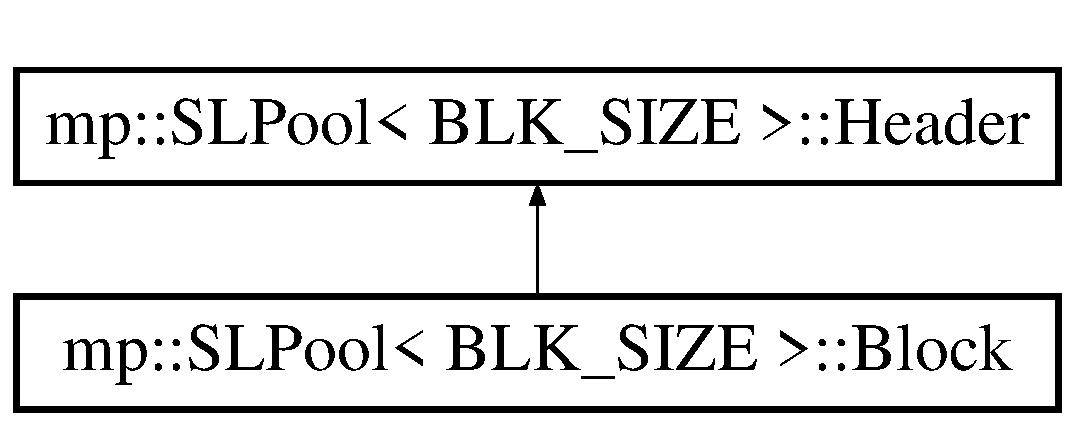
\includegraphics[height=2.000000cm]{structmp_1_1_s_l_pool_1_1_block}
\end{center}
\end{figure}
\subsection*{Public Member Functions}
\begin{DoxyCompactItemize}
\item 
\hyperlink{structmp_1_1_s_l_pool_1_1_block_a05fd1764262649601dd90385c8701779}{Block} ()
\end{DoxyCompactItemize}
\subsection*{Public Attributes}
\begin{DoxyCompactItemize}
\item 
\begin{tabbing}
xx\=xx\=xx\=xx\=xx\=xx\=xx\=xx\=xx\=\kill
union \{\\
\hyperlink{structmp_1_1_s_l_pool_1_1_block}{Block} $\ast$ {\bfseries m\_next}\\
char {\bfseries m\_raw} \mbox{[}BLK\_SIZE -\/ sizeof(\hyperlink{structmp_1_1_s_l_pool_1_1_header}{Header})\mbox{]}\\
\}; \\

\end{tabbing}\end{DoxyCompactItemize}


\subsection{Constructor \& Destructor Documentation}
\mbox{\Hypertarget{structmp_1_1_s_l_pool_1_1_block_a05fd1764262649601dd90385c8701779}\label{structmp_1_1_s_l_pool_1_1_block_a05fd1764262649601dd90385c8701779}} 
\index{mp\+::\+S\+L\+Pool\+::\+Block@{mp\+::\+S\+L\+Pool\+::\+Block}!Block@{Block}}
\index{Block@{Block}!mp\+::\+S\+L\+Pool\+::\+Block@{mp\+::\+S\+L\+Pool\+::\+Block}}
\subsubsection{\texorpdfstring{Block()}{Block()}}
{\footnotesize\ttfamily template$<$size\+\_\+t B\+L\+K\+\_\+\+S\+I\+ZE = 16$>$ \\
\hyperlink{classmp_1_1_s_l_pool}{mp\+::\+S\+L\+Pool}$<$ B\+L\+K\+\_\+\+S\+I\+ZE $>$\+::Block\+::\+Block (\begin{DoxyParamCaption}{ }\end{DoxyParamCaption})\hspace{0.3cm}{\ttfamily [inline]}}



\subsection{Member Data Documentation}
\mbox{\Hypertarget{structmp_1_1_s_l_pool_1_1_block_a16dc0abe30900180b814ba2212a6ea9c}\label{structmp_1_1_s_l_pool_1_1_block_a16dc0abe30900180b814ba2212a6ea9c}} 
\subsubsection{\texorpdfstring{"@1}{@1}}
{\footnotesize\ttfamily union \{ ... \} }


\hypertarget{structmp_1_1_s_l_pool_1_1_header}{}\section{mp\+:\+:S\+L\+Pool$<$ B\+L\+K\+\_\+\+S\+I\+ZE $>$\+:\+:Header Struct Reference}
\label{structmp_1_1_s_l_pool_1_1_header}\index{mp\+::\+S\+L\+Pool$<$ B\+L\+K\+\_\+\+S\+I\+Z\+E $>$\+::\+Header@{mp\+::\+S\+L\+Pool$<$ B\+L\+K\+\_\+\+S\+I\+Z\+E $>$\+::\+Header}}
Inheritance diagram for mp\+:\+:S\+L\+Pool$<$ B\+L\+K\+\_\+\+S\+I\+ZE $>$\+:\+:Header\+:\begin{figure}[H]
\begin{center}
\leavevmode
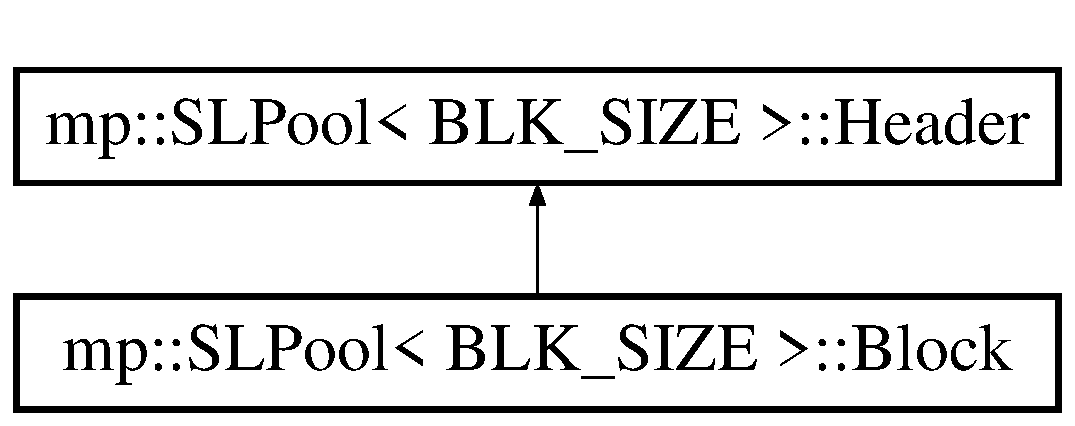
\includegraphics[height=2.000000cm]{structmp_1_1_s_l_pool_1_1_header}
\end{center}
\end{figure}
\subsection*{Public Member Functions}
\begin{DoxyCompactItemize}
\item 
\hyperlink{structmp_1_1_s_l_pool_1_1_header_a8dde5a9b243239f67fa13cbc63fce081}{Header} ()
\end{DoxyCompactItemize}
\subsection*{Public Attributes}
\begin{DoxyCompactItemize}
\item 
size\+\_\+t \hyperlink{structmp_1_1_s_l_pool_1_1_header_a4ce73cd63134fdeb85adab3c35b744c0}{m\+\_\+length}
\end{DoxyCompactItemize}


\subsection{Constructor \& Destructor Documentation}
\mbox{\Hypertarget{structmp_1_1_s_l_pool_1_1_header_a8dde5a9b243239f67fa13cbc63fce081}\label{structmp_1_1_s_l_pool_1_1_header_a8dde5a9b243239f67fa13cbc63fce081}} 
\index{mp\+::\+S\+L\+Pool\+::\+Header@{mp\+::\+S\+L\+Pool\+::\+Header}!Header@{Header}}
\index{Header@{Header}!mp\+::\+S\+L\+Pool\+::\+Header@{mp\+::\+S\+L\+Pool\+::\+Header}}
\subsubsection{\texorpdfstring{Header()}{Header()}}
{\footnotesize\ttfamily template$<$size\+\_\+t B\+L\+K\+\_\+\+S\+I\+ZE = 16$>$ \\
\hyperlink{classmp_1_1_s_l_pool}{mp\+::\+S\+L\+Pool}$<$ B\+L\+K\+\_\+\+S\+I\+ZE $>$\+::Header\+::\+Header (\begin{DoxyParamCaption}{ }\end{DoxyParamCaption})\hspace{0.3cm}{\ttfamily [inline]}}



\subsection{Member Data Documentation}
\mbox{\Hypertarget{structmp_1_1_s_l_pool_1_1_header_a4ce73cd63134fdeb85adab3c35b744c0}\label{structmp_1_1_s_l_pool_1_1_header_a4ce73cd63134fdeb85adab3c35b744c0}} 
\index{mp\+::\+S\+L\+Pool\+::\+Header@{mp\+::\+S\+L\+Pool\+::\+Header}!m\+\_\+length@{m\+\_\+length}}
\index{m\+\_\+length@{m\+\_\+length}!mp\+::\+S\+L\+Pool\+::\+Header@{mp\+::\+S\+L\+Pool\+::\+Header}}
\subsubsection{\texorpdfstring{m\+\_\+length}{m\_length}}
{\footnotesize\ttfamily template$<$size\+\_\+t B\+L\+K\+\_\+\+S\+I\+ZE = 16$>$ \\
size\+\_\+t \hyperlink{classmp_1_1_s_l_pool}{mp\+::\+S\+L\+Pool}$<$ B\+L\+K\+\_\+\+S\+I\+ZE $>$\+::Header\+::m\+\_\+length}


\hypertarget{classmp_1_1_s_l_pool}{}\section{mp\+:\+:S\+L\+Pool$<$ B\+L\+K\+\_\+\+S\+I\+ZE $>$ Class Template Reference}
\label{classmp_1_1_s_l_pool}\index{mp\+::\+S\+L\+Pool$<$ B\+L\+K\+\_\+\+S\+I\+Z\+E $>$@{mp\+::\+S\+L\+Pool$<$ B\+L\+K\+\_\+\+S\+I\+Z\+E $>$}}
Inheritance diagram for mp\+:\+:S\+L\+Pool$<$ B\+L\+K\+\_\+\+S\+I\+ZE $>$\+:\begin{figure}[H]
\begin{center}
\leavevmode
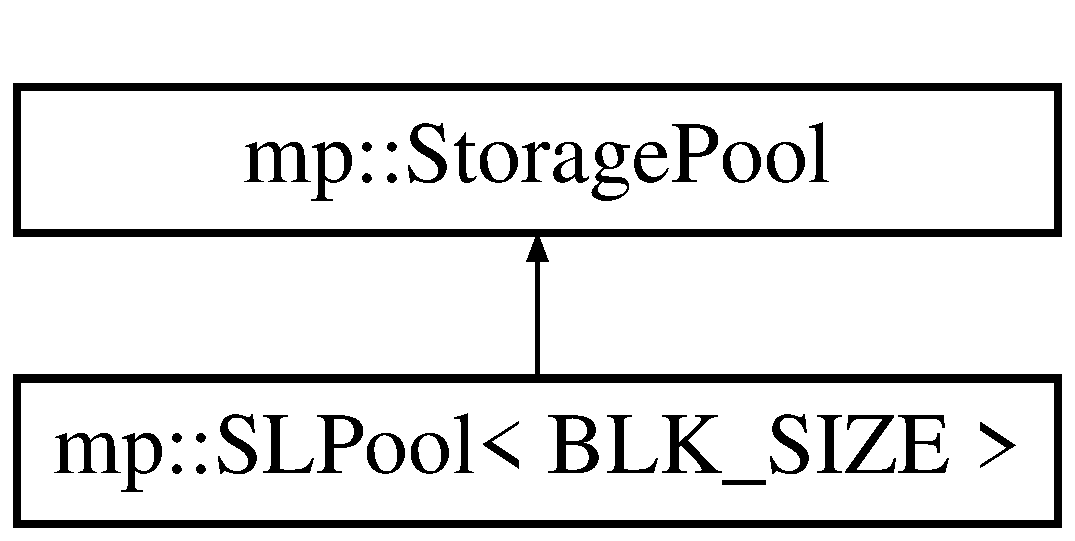
\includegraphics[height=2.000000cm]{classmp_1_1_s_l_pool}
\end{center}
\end{figure}
\subsection*{Classes}
\begin{DoxyCompactItemize}
\item 
struct \hyperlink{structmp_1_1_s_l_pool_1_1_block}{Block}
\item 
union \hyperlink{classmp_1_1_s_l_pool_unionmp_1_1_s_l_pool_1_1_block_8____unnamed____}{Block.\+\_\+\+\_\+unnamed\+\_\+\+\_\+}
\item 
struct \hyperlink{structmp_1_1_s_l_pool_1_1_header}{Header}
\end{DoxyCompactItemize}
\subsection*{Public Member Functions}
\begin{DoxyCompactItemize}
\item 
\hyperlink{classmp_1_1_s_l_pool_a9f1a91197f85fac54d0ed7f4f2d53b6e}{S\+L\+Pool} (size\+\_\+t mem)
\item 
\hyperlink{classmp_1_1_s_l_pool_ab1a395b720c1f1bc3d87b43346200695}{$\sim$\+S\+L\+Pool} ()
\item 
void $\ast$ \hyperlink{classmp_1_1_s_l_pool_a543f5c4b2d190bbfc89170a227dc92a8}{Allocate} (size\+\_\+t mem)
\item 
void \hyperlink{classmp_1_1_s_l_pool_a605b83d9042098aabaf19e3796222a74}{Free} (void $\ast$pt\+\_\+m)
\item 
void \hyperlink{classmp_1_1_s_l_pool_a6770602574612fd2ef47bf474c0797bc}{visualisation} ()
\end{DoxyCompactItemize}
\subsection*{Static Public Attributes}
\begin{DoxyCompactItemize}
\item 
static constexpr size\+\_\+t \hyperlink{classmp_1_1_s_l_pool_a9713b7eaf26afed603cab879a2144dbf}{B\+L\+K\+\_\+\+SZ} = sizeof( \hyperlink{classmp_1_1_s_l_pool}{mp\+::\+S\+L\+Pool}$<$B\+L\+K\+\_\+\+S\+I\+ZE$>$\+::\hyperlink{structmp_1_1_s_l_pool_1_1_block}{Block} )
\begin{DoxyCompactList}\small\item\em The block size in bytes. \end{DoxyCompactList}\item 
static constexpr size\+\_\+t \hyperlink{classmp_1_1_s_l_pool_aa43372c95c4efa9d0609e6338d5ffacd}{T\+A\+G\+\_\+\+SZ} = sizeof( \hyperlink{namespacemp_structmp_1_1_tag}{mp\+::\+Tag} )
\begin{DoxyCompactList}\small\item\em The \hyperlink{namespacemp_structmp_1_1_tag}{Tag} size in bytes (each reserved area has a tag). \end{DoxyCompactList}\item 
static constexpr size\+\_\+t \hyperlink{classmp_1_1_s_l_pool_a6a08294207c41778969fa9316e1374dc}{H\+E\+A\+D\+E\+R\+\_\+\+SZ} = sizeof( \hyperlink{classmp_1_1_s_l_pool}{mp\+::\+S\+L\+Pool}$<$B\+L\+K\+\_\+\+S\+I\+ZE$>$\+::\hyperlink{structmp_1_1_s_l_pool_1_1_header}{Header} )
\begin{DoxyCompactList}\small\item\em The header size in bytes. \end{DoxyCompactList}\end{DoxyCompactItemize}
\subsection*{Private Attributes}
\begin{DoxyCompactItemize}
\item 
unsigned int \hyperlink{classmp_1_1_s_l_pool_ad0aad2c91ed55f7ce1e2f8c3da37006d}{m\+\_\+n\+\_\+blocks}
\begin{DoxyCompactList}\small\item\em Number of blocks in the list. \end{DoxyCompactList}\item 
\hyperlink{structmp_1_1_s_l_pool_1_1_block}{Block} $\ast$ \hyperlink{classmp_1_1_s_l_pool_a27f201ccadbf0bddca5ccc53473bde39}{m\+\_\+pool}
\begin{DoxyCompactList}\small\item\em Head of list. \end{DoxyCompactList}\item 
\hyperlink{structmp_1_1_s_l_pool_1_1_block}{Block} \& \hyperlink{classmp_1_1_s_l_pool_a3c3858050e1ca40c314ae8cfd3612d38}{m\+\_\+sentinel}
\begin{DoxyCompactList}\small\item\em End of the list. \end{DoxyCompactList}\end{DoxyCompactItemize}


\subsection{Class Documentation}
\index{mp\+::\+S\+L\+Pool\+::\+Block.\+\_\+\+\_\+unnamed\+\_\+\+\_\+@{mp\+::\+S\+L\+Pool\+::\+Block.\+\_\+\+\_\+unnamed\+\_\+\+\_\+}}\label{unionmp_1_1_s_l_pool_1_1_block_8____unnamed____}
\Hypertarget{classmp_1_1_s_l_pool_unionmp_1_1_s_l_pool_1_1_block_8____unnamed____}
\subsubsection{union mp\+:\+:S\+L\+Pool\+:\+:Block.\+\_\+\+\_\+unnamed\+\_\+\+\_\+}
\subsubsection*{template$<$size\+\_\+t B\+L\+K\+\_\+\+S\+I\+ZE = 16$>$\newline
union mp\+::\+S\+L\+Pool$<$ B\+L\+K\+\_\+\+S\+I\+Z\+E $>$\+::\+Block.\+\_\+\+\_\+unnamed\+\_\+\+\_\+}

\begin{DoxyFields}{Class Members}
\mbox{\Hypertarget{classmp_1_1_s_l_pool_a3bfb47e8362544e4462b7fae503e3774}\label{classmp_1_1_s_l_pool_a3bfb47e8362544e4462b7fae503e3774}} 
\hyperlink{structmp_1_1_s_l_pool_1_1_block}{Block} $\ast$&
m\_next&
\\
\hline

\mbox{\Hypertarget{classmp_1_1_s_l_pool_a380f5cc05b47f6bb73d4b4c8ccd91090}\label{classmp_1_1_s_l_pool_a380f5cc05b47f6bb73d4b4c8ccd91090}} 
char&
m\_raw\mbox{[}BLK\_SIZE -\/ sizeof(\hyperlink{structmp_1_1_s_l_pool_1_1_header}{Header})\mbox{]}&
\\
\hline

\end{DoxyFields}


\subsection{Constructor \& Destructor Documentation}
\mbox{\Hypertarget{classmp_1_1_s_l_pool_a9f1a91197f85fac54d0ed7f4f2d53b6e}\label{classmp_1_1_s_l_pool_a9f1a91197f85fac54d0ed7f4f2d53b6e}} 
\index{mp\+::\+S\+L\+Pool@{mp\+::\+S\+L\+Pool}!S\+L\+Pool@{S\+L\+Pool}}
\index{S\+L\+Pool@{S\+L\+Pool}!mp\+::\+S\+L\+Pool@{mp\+::\+S\+L\+Pool}}
\subsubsection{\texorpdfstring{S\+L\+Pool()}{SLPool()}}
{\footnotesize\ttfamily template$<$size\+\_\+t B\+L\+K\+\_\+\+S\+I\+ZE = 16$>$ \\
\hyperlink{classmp_1_1_s_l_pool}{mp\+::\+S\+L\+Pool}$<$ B\+L\+K\+\_\+\+S\+I\+ZE $>$\+::\hyperlink{classmp_1_1_s_l_pool}{S\+L\+Pool} (\begin{DoxyParamCaption}\item[{size\+\_\+t}]{mem }\end{DoxyParamCaption})\hspace{0.3cm}{\ttfamily [inline]}, {\ttfamily [explicit]}}

$<$ Size of the free space.

$<$ Pointer to next node.

$<$ pointer to first node.

$<$ Sentinel size. \mbox{\Hypertarget{classmp_1_1_s_l_pool_ab1a395b720c1f1bc3d87b43346200695}\label{classmp_1_1_s_l_pool_ab1a395b720c1f1bc3d87b43346200695}} 
\index{mp\+::\+S\+L\+Pool@{mp\+::\+S\+L\+Pool}!````~S\+L\+Pool@{$\sim$\+S\+L\+Pool}}
\index{````~S\+L\+Pool@{$\sim$\+S\+L\+Pool}!mp\+::\+S\+L\+Pool@{mp\+::\+S\+L\+Pool}}
\subsubsection{\texorpdfstring{$\sim$\+S\+L\+Pool()}{~SLPool()}}
{\footnotesize\ttfamily template$<$size\+\_\+t B\+L\+K\+\_\+\+S\+I\+ZE = 16$>$ \\
\hyperlink{classmp_1_1_s_l_pool}{mp\+::\+S\+L\+Pool}$<$ B\+L\+K\+\_\+\+S\+I\+ZE $>$\+::$\sim$\hyperlink{classmp_1_1_s_l_pool}{S\+L\+Pool} (\begin{DoxyParamCaption}{ }\end{DoxyParamCaption})\hspace{0.3cm}{\ttfamily [inline]}}



\subsection{Member Function Documentation}
\mbox{\Hypertarget{classmp_1_1_s_l_pool_a543f5c4b2d190bbfc89170a227dc92a8}\label{classmp_1_1_s_l_pool_a543f5c4b2d190bbfc89170a227dc92a8}} 
\index{mp\+::\+S\+L\+Pool@{mp\+::\+S\+L\+Pool}!Allocate@{Allocate}}
\index{Allocate@{Allocate}!mp\+::\+S\+L\+Pool@{mp\+::\+S\+L\+Pool}}
\subsubsection{\texorpdfstring{Allocate()}{Allocate()}}
{\footnotesize\ttfamily template$<$size\+\_\+t B\+L\+K\+\_\+\+S\+I\+ZE = 16$>$ \\
void$\ast$ \hyperlink{classmp_1_1_s_l_pool}{mp\+::\+S\+L\+Pool}$<$ B\+L\+K\+\_\+\+S\+I\+ZE $>$\+::Allocate (\begin{DoxyParamCaption}\item[{size\+\_\+t}]{mem }\end{DoxyParamCaption})\hspace{0.3cm}{\ttfamily [inline]}, {\ttfamily [virtual]}}

$<$ Pointer to the first node.

$<$ Pointer to the sentinel

$<$ the number of blocks that will be used.

$<$ If dont need to create a new node of free blocks.

$<$ Updating the pointer to other head.

$<$ Size of the raw space.

$<$ Updating the old pointer.

$<$ Updating the new node pointer.

$<$ Updating the space of the new node.

$<$ Size of the raw space.

$<$ Updating the pointer to next posicion.

$<$ Updating the pointer to next posicion. 
\begin{DoxyParams}{Parameters}
{\em mem} & Allocate a raw using First-\/fit. \\
\hline
\end{DoxyParams}


Implements \hyperlink{classmp_1_1_storage_pool_a7970f46f34c0e532544888ecaf10b4c9}{mp\+::\+Storage\+Pool}.

\mbox{\Hypertarget{classmp_1_1_s_l_pool_a605b83d9042098aabaf19e3796222a74}\label{classmp_1_1_s_l_pool_a605b83d9042098aabaf19e3796222a74}} 
\index{mp\+::\+S\+L\+Pool@{mp\+::\+S\+L\+Pool}!Free@{Free}}
\index{Free@{Free}!mp\+::\+S\+L\+Pool@{mp\+::\+S\+L\+Pool}}
\subsubsection{\texorpdfstring{Free()}{Free()}}
{\footnotesize\ttfamily template$<$size\+\_\+t B\+L\+K\+\_\+\+S\+I\+ZE = 16$>$ \\
void \hyperlink{classmp_1_1_s_l_pool}{mp\+::\+S\+L\+Pool}$<$ B\+L\+K\+\_\+\+S\+I\+ZE $>$\+::Free (\begin{DoxyParamCaption}\item[{void $\ast$}]{pt\+\_\+m }\end{DoxyParamCaption})\hspace{0.3cm}{\ttfamily [inline]}, {\ttfamily [virtual]}}

$<$ Pointer to raw area that will be released.

$<$ Pointer to position node after the raw area.

$<$ Pinter to node before the raw.

$<$ Updating the pointers to left and right position.

$<$ Checking if the raw area have free adjacent areas.

$<$ Making a uniq pointer to the next block.

$<$ Unite the three length spaces.

$<$ Checking if the right area is a free adjacent area.

$<$ Making a uniq pointer to the next block.

$<$ Unite the two length spaces.

$<$ Checking if the left area is a free adjacent area.

$<$ Unite the two length spaces.

$<$ Checking if the raw area dont have free adjacent areas.

$<$ Making a pointer to the next node. 
\begin{DoxyParams}{Parameters}
{\em pt\+\_\+m} & free a raw area. \\
\hline
\end{DoxyParams}


Implements \hyperlink{classmp_1_1_storage_pool_a5a186404980f6c958a30373f810ebd4f}{mp\+::\+Storage\+Pool}.

\mbox{\Hypertarget{classmp_1_1_s_l_pool_a6770602574612fd2ef47bf474c0797bc}\label{classmp_1_1_s_l_pool_a6770602574612fd2ef47bf474c0797bc}} 
\index{mp\+::\+S\+L\+Pool@{mp\+::\+S\+L\+Pool}!visualisation@{visualisation}}
\index{visualisation@{visualisation}!mp\+::\+S\+L\+Pool@{mp\+::\+S\+L\+Pool}}
\subsubsection{\texorpdfstring{visualisation()}{visualisation()}}
{\footnotesize\ttfamily template$<$size\+\_\+t B\+L\+K\+\_\+\+S\+I\+ZE = 16$>$ \\
void \hyperlink{classmp_1_1_s_l_pool}{mp\+::\+S\+L\+Pool}$<$ B\+L\+K\+\_\+\+S\+I\+ZE $>$\+::visualisation (\begin{DoxyParamCaption}{ }\end{DoxyParamCaption})\hspace{0.3cm}{\ttfamily [inline]}}

$<$ Pointer to position node after the raw area. 

\subsection{Member Data Documentation}
\mbox{\Hypertarget{classmp_1_1_s_l_pool_a9713b7eaf26afed603cab879a2144dbf}\label{classmp_1_1_s_l_pool_a9713b7eaf26afed603cab879a2144dbf}} 
\index{mp\+::\+S\+L\+Pool@{mp\+::\+S\+L\+Pool}!B\+L\+K\+\_\+\+SZ@{B\+L\+K\+\_\+\+SZ}}
\index{B\+L\+K\+\_\+\+SZ@{B\+L\+K\+\_\+\+SZ}!mp\+::\+S\+L\+Pool@{mp\+::\+S\+L\+Pool}}
\subsubsection{\texorpdfstring{B\+L\+K\+\_\+\+SZ}{BLK\_SZ}}
{\footnotesize\ttfamily template$<$size\+\_\+t B\+L\+K\+\_\+\+S\+I\+ZE = 16$>$ \\
constexpr size\+\_\+t \hyperlink{classmp_1_1_s_l_pool}{mp\+::\+S\+L\+Pool}$<$ B\+L\+K\+\_\+\+S\+I\+ZE $>$\+::B\+L\+K\+\_\+\+SZ = sizeof( \hyperlink{classmp_1_1_s_l_pool}{mp\+::\+S\+L\+Pool}$<$B\+L\+K\+\_\+\+S\+I\+ZE$>$\+::\hyperlink{structmp_1_1_s_l_pool_1_1_block}{Block} )\hspace{0.3cm}{\ttfamily [static]}}



The block size in bytes. 

\mbox{\Hypertarget{classmp_1_1_s_l_pool_a6a08294207c41778969fa9316e1374dc}\label{classmp_1_1_s_l_pool_a6a08294207c41778969fa9316e1374dc}} 
\index{mp\+::\+S\+L\+Pool@{mp\+::\+S\+L\+Pool}!H\+E\+A\+D\+E\+R\+\_\+\+SZ@{H\+E\+A\+D\+E\+R\+\_\+\+SZ}}
\index{H\+E\+A\+D\+E\+R\+\_\+\+SZ@{H\+E\+A\+D\+E\+R\+\_\+\+SZ}!mp\+::\+S\+L\+Pool@{mp\+::\+S\+L\+Pool}}
\subsubsection{\texorpdfstring{H\+E\+A\+D\+E\+R\+\_\+\+SZ}{HEADER\_SZ}}
{\footnotesize\ttfamily template$<$size\+\_\+t B\+L\+K\+\_\+\+S\+I\+ZE = 16$>$ \\
constexpr size\+\_\+t \hyperlink{classmp_1_1_s_l_pool}{mp\+::\+S\+L\+Pool}$<$ B\+L\+K\+\_\+\+S\+I\+ZE $>$\+::H\+E\+A\+D\+E\+R\+\_\+\+SZ = sizeof( \hyperlink{classmp_1_1_s_l_pool}{mp\+::\+S\+L\+Pool}$<$B\+L\+K\+\_\+\+S\+I\+ZE$>$\+::\hyperlink{structmp_1_1_s_l_pool_1_1_header}{Header} )\hspace{0.3cm}{\ttfamily [static]}}



The header size in bytes. 

\mbox{\Hypertarget{classmp_1_1_s_l_pool_ad0aad2c91ed55f7ce1e2f8c3da37006d}\label{classmp_1_1_s_l_pool_ad0aad2c91ed55f7ce1e2f8c3da37006d}} 
\index{mp\+::\+S\+L\+Pool@{mp\+::\+S\+L\+Pool}!m\+\_\+n\+\_\+blocks@{m\+\_\+n\+\_\+blocks}}
\index{m\+\_\+n\+\_\+blocks@{m\+\_\+n\+\_\+blocks}!mp\+::\+S\+L\+Pool@{mp\+::\+S\+L\+Pool}}
\subsubsection{\texorpdfstring{m\+\_\+n\+\_\+blocks}{m\_n\_blocks}}
{\footnotesize\ttfamily template$<$size\+\_\+t B\+L\+K\+\_\+\+S\+I\+ZE = 16$>$ \\
unsigned int \hyperlink{classmp_1_1_s_l_pool}{mp\+::\+S\+L\+Pool}$<$ B\+L\+K\+\_\+\+S\+I\+ZE $>$\+::m\+\_\+n\+\_\+blocks\hspace{0.3cm}{\ttfamily [private]}}



Number of blocks in the list. 

\mbox{\Hypertarget{classmp_1_1_s_l_pool_a27f201ccadbf0bddca5ccc53473bde39}\label{classmp_1_1_s_l_pool_a27f201ccadbf0bddca5ccc53473bde39}} 
\index{mp\+::\+S\+L\+Pool@{mp\+::\+S\+L\+Pool}!m\+\_\+pool@{m\+\_\+pool}}
\index{m\+\_\+pool@{m\+\_\+pool}!mp\+::\+S\+L\+Pool@{mp\+::\+S\+L\+Pool}}
\subsubsection{\texorpdfstring{m\+\_\+pool}{m\_pool}}
{\footnotesize\ttfamily template$<$size\+\_\+t B\+L\+K\+\_\+\+S\+I\+ZE = 16$>$ \\
\hyperlink{structmp_1_1_s_l_pool_1_1_block}{Block}$\ast$ \hyperlink{classmp_1_1_s_l_pool}{mp\+::\+S\+L\+Pool}$<$ B\+L\+K\+\_\+\+S\+I\+ZE $>$\+::m\+\_\+pool\hspace{0.3cm}{\ttfamily [private]}}



Head of list. 

\mbox{\Hypertarget{classmp_1_1_s_l_pool_a3c3858050e1ca40c314ae8cfd3612d38}\label{classmp_1_1_s_l_pool_a3c3858050e1ca40c314ae8cfd3612d38}} 
\index{mp\+::\+S\+L\+Pool@{mp\+::\+S\+L\+Pool}!m\+\_\+sentinel@{m\+\_\+sentinel}}
\index{m\+\_\+sentinel@{m\+\_\+sentinel}!mp\+::\+S\+L\+Pool@{mp\+::\+S\+L\+Pool}}
\subsubsection{\texorpdfstring{m\+\_\+sentinel}{m\_sentinel}}
{\footnotesize\ttfamily template$<$size\+\_\+t B\+L\+K\+\_\+\+S\+I\+ZE = 16$>$ \\
\hyperlink{structmp_1_1_s_l_pool_1_1_block}{Block}\& \hyperlink{classmp_1_1_s_l_pool}{mp\+::\+S\+L\+Pool}$<$ B\+L\+K\+\_\+\+S\+I\+ZE $>$\+::m\+\_\+sentinel\hspace{0.3cm}{\ttfamily [private]}}



End of the list. 

\mbox{\Hypertarget{classmp_1_1_s_l_pool_aa43372c95c4efa9d0609e6338d5ffacd}\label{classmp_1_1_s_l_pool_aa43372c95c4efa9d0609e6338d5ffacd}} 
\index{mp\+::\+S\+L\+Pool@{mp\+::\+S\+L\+Pool}!T\+A\+G\+\_\+\+SZ@{T\+A\+G\+\_\+\+SZ}}
\index{T\+A\+G\+\_\+\+SZ@{T\+A\+G\+\_\+\+SZ}!mp\+::\+S\+L\+Pool@{mp\+::\+S\+L\+Pool}}
\subsubsection{\texorpdfstring{T\+A\+G\+\_\+\+SZ}{TAG\_SZ}}
{\footnotesize\ttfamily template$<$size\+\_\+t B\+L\+K\+\_\+\+S\+I\+ZE = 16$>$ \\
constexpr size\+\_\+t \hyperlink{classmp_1_1_s_l_pool}{mp\+::\+S\+L\+Pool}$<$ B\+L\+K\+\_\+\+S\+I\+ZE $>$\+::T\+A\+G\+\_\+\+SZ = sizeof( \hyperlink{namespacemp_structmp_1_1_tag}{mp\+::\+Tag} )\hspace{0.3cm}{\ttfamily [static]}}



The \hyperlink{namespacemp_structmp_1_1_tag}{Tag} size in bytes (each reserved area has a tag). 


\hypertarget{classmp_1_1_storage_pool}{}\section{mp\+:\+:Storage\+Pool Class Reference}
\label{classmp_1_1_storage_pool}\index{mp\+::\+Storage\+Pool@{mp\+::\+Storage\+Pool}}
Inheritance diagram for mp\+:\+:Storage\+Pool\+:\begin{figure}[H]
\begin{center}
\leavevmode
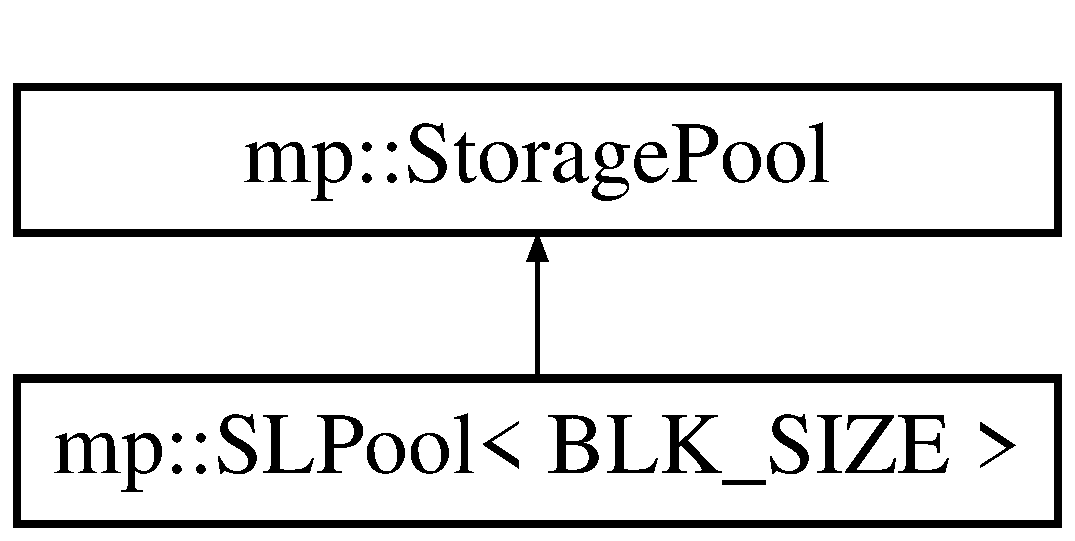
\includegraphics[height=2.000000cm]{classmp_1_1_storage_pool}
\end{center}
\end{figure}
\subsection*{Public Member Functions}
\begin{DoxyCompactItemize}
\item 
virtual \hyperlink{classmp_1_1_storage_pool_a832cd1b08193b04194adb81d0eea7ca3}{$\sim$\+Storage\+Pool} ()
\item 
virtual void $\ast$ \hyperlink{classmp_1_1_storage_pool_a7970f46f34c0e532544888ecaf10b4c9}{Allocate} (size\+\_\+t)=0
\item 
virtual void \hyperlink{classmp_1_1_storage_pool_a5a186404980f6c958a30373f810ebd4f}{Free} (void $\ast$)=0
\end{DoxyCompactItemize}


\subsection{Constructor \& Destructor Documentation}
\mbox{\Hypertarget{classmp_1_1_storage_pool_a832cd1b08193b04194adb81d0eea7ca3}\label{classmp_1_1_storage_pool_a832cd1b08193b04194adb81d0eea7ca3}} 
\index{mp\+::\+Storage\+Pool@{mp\+::\+Storage\+Pool}!````~Storage\+Pool@{$\sim$\+Storage\+Pool}}
\index{````~Storage\+Pool@{$\sim$\+Storage\+Pool}!mp\+::\+Storage\+Pool@{mp\+::\+Storage\+Pool}}
\subsubsection{\texorpdfstring{$\sim$\+Storage\+Pool()}{~StoragePool()}}
{\footnotesize\ttfamily virtual mp\+::\+Storage\+Pool\+::$\sim$\+Storage\+Pool (\begin{DoxyParamCaption}{ }\end{DoxyParamCaption})\hspace{0.3cm}{\ttfamily [inline]}, {\ttfamily [virtual]}}



\subsection{Member Function Documentation}
\mbox{\Hypertarget{classmp_1_1_storage_pool_a7970f46f34c0e532544888ecaf10b4c9}\label{classmp_1_1_storage_pool_a7970f46f34c0e532544888ecaf10b4c9}} 
\index{mp\+::\+Storage\+Pool@{mp\+::\+Storage\+Pool}!Allocate@{Allocate}}
\index{Allocate@{Allocate}!mp\+::\+Storage\+Pool@{mp\+::\+Storage\+Pool}}
\subsubsection{\texorpdfstring{Allocate()}{Allocate()}}
{\footnotesize\ttfamily virtual void$\ast$ mp\+::\+Storage\+Pool\+::\+Allocate (\begin{DoxyParamCaption}\item[{size\+\_\+t}]{ }\end{DoxyParamCaption})\hspace{0.3cm}{\ttfamily [pure virtual]}}



Implemented in \hyperlink{classmp_1_1_s_l_pool_a543f5c4b2d190bbfc89170a227dc92a8}{mp\+::\+S\+L\+Pool$<$ B\+L\+K\+\_\+\+S\+I\+Z\+E $>$}.

\mbox{\Hypertarget{classmp_1_1_storage_pool_a5a186404980f6c958a30373f810ebd4f}\label{classmp_1_1_storage_pool_a5a186404980f6c958a30373f810ebd4f}} 
\index{mp\+::\+Storage\+Pool@{mp\+::\+Storage\+Pool}!Free@{Free}}
\index{Free@{Free}!mp\+::\+Storage\+Pool@{mp\+::\+Storage\+Pool}}
\subsubsection{\texorpdfstring{Free()}{Free()}}
{\footnotesize\ttfamily virtual void mp\+::\+Storage\+Pool\+::\+Free (\begin{DoxyParamCaption}\item[{void $\ast$}]{ }\end{DoxyParamCaption})\hspace{0.3cm}{\ttfamily [pure virtual]}}



Implemented in \hyperlink{classmp_1_1_s_l_pool_a605b83d9042098aabaf19e3796222a74}{mp\+::\+S\+L\+Pool$<$ B\+L\+K\+\_\+\+S\+I\+Z\+E $>$}.


%--- End generated contents ---

% Index
\backmatter
\newpage
\phantomsection
\clearemptydoublepage
\addcontentsline{toc}{chapter}{Index}
\printindex

\end{document}
